% !TeX root = ..\rapport_13_2.tex
\section{Design mønstre} \label{chap:design}
Der har været fokus på at adskille præsentationslag, businesslag, og persistence-lag og flere design mønstre er anvendt for at opnå et let læseligt, overskueligt og lavt koblet system. 

\subsection{Program-lag}
Et fuldt klassediagram over program-laget kan ses i appendix \ref{apdx:classDiagram_full}. Et simplificeret klassediagram herunder i \ref{fig:class_persistency_layer} viser relationer mellem klasserne i TaskFusion programmet. TaskFusion fungere som hovedklasse og er primært ansvarlig for brugergodkendelser. Et facade mønster (eng: Facade pattern) er implementeret med \texttt{EmployeeFacade.java} og \texttt{ProjectFacade.java} for at opnå lav kobling. F.eks. bliver systemet, der behandler employees, tilgået gennem \texttt{EmployeeFacade.java} således at klasserne, bestående af bl.a. \texttt{EmployeeRepository.java}, \texttt{Employee.java}, \texttt{RegularActivity.java}, ikke skal kaldes af klienten på forskellig vis. I stedet kan klienten tilgå alle de nødvendige egenskaber igennem facaden kun. Sammen med \textit{EmployeeFacade} og \textit{ProjectFacade} eksponere \textit{TaskFusion} de offentlige metoder der skal kunne tilgås i programmet. På den måde kan vi frihed til at ændre alle metoder i de resterende program-lag, uden det vil påvirke eventuelle brugergrænseflader. Alle metoder i \textit{facade} klasserne kan i virkeligheden ligge i TaskFusion klassen, men ved at opdele metoderne i passende seperate klasser, kan vi bedre vedligeholde og udbygge programmet. 
Programmets domæne lag består af instantierbare objektklasser og er ansvarlig for \textit{Business-logic}. Persistency-laget indeholder \textit{Repositories}, der er ansvarlige for kommunikation med en lagringsløsning. Selvom programmet ikke har et database lag på nuværende tidspunkt, vil det være let at bygge flere lagringsløsninger på senere, ved kun at skulle modificere persistency klasserne. 

\begin{figure}[H]
    \centering
    \caption{Klassediagram over program-lag}
    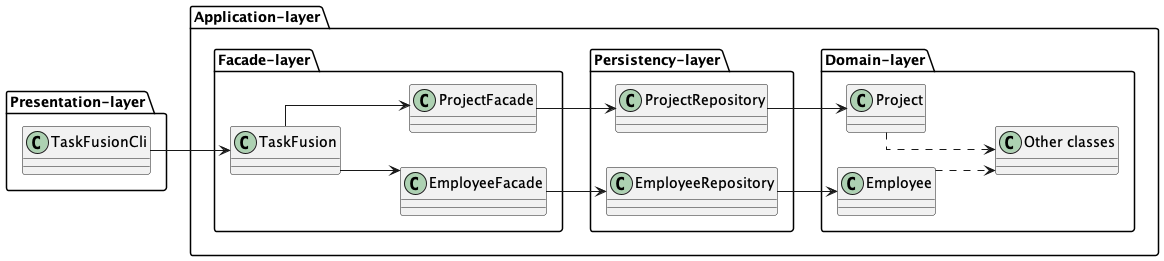
\includegraphics[width = \textwidth, keepaspectratio]{TaskFusion/out/assets/diagrams/class_persistency_layer/ClassDiagram_layer.png}
    \label{fig:class_persistency_layer}
\end{figure}

Vi ønsker desuden aldrig at eksponere programmets klasser udenfor program-laget. Derfor implementere alle instantierbare klasser i domæne-laget \textit{ConvertibleToViewModel}-interfacet, vist herunder i \ref{fig:class_persistency_domain}. Dette interface kræver at klasserne kan eksporteres til en tilsvarende visningsklasse til brug i præsentations-lag. På den måde kan vi undgå at brugere kan kalde metoder fra domæne-laget, og dermed sikre de forudsætninger de enkelte metoder måtte have.

\begin{figure}[H]
    \centering
    \caption{Domæne-laget}
    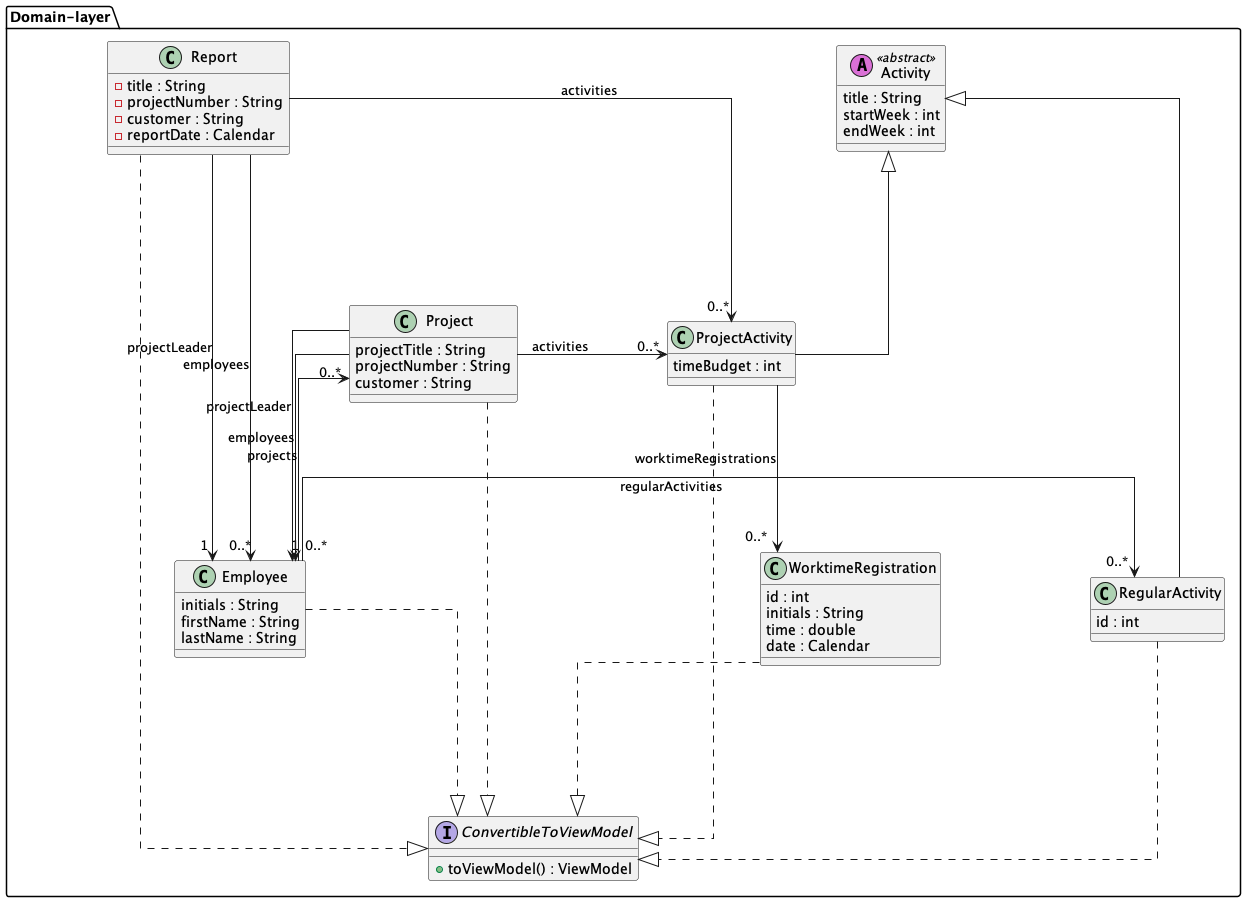
\includegraphics[width = \textwidth, keepaspectratio]{TaskFusion/out/assets/diagrams/class_persistency_domain/ClassDiagram_domain.png}
    \label{fig:class_persistency_domain}
\end{figure}

Et andet design mønster der er taget i brug, er singleton design mønstret. F.eks. haves et opbevaringssted for alle medarbejdere kaldet \textit{EmployeeRepository}. Der ønskes kun én instans af dette objekt, da idéen er at tilgå og opbevare medarbejderne via. ét objekt. Hvis flere instanser af dette objekt skulle forekomme, er det ikke sikret, at brugeren kan tilgå alle medarbejderne fra den ene instans, da medarbejdere kan eksistere i de andre instanser, hvorfor objektet skal være en singleton. Af samme grunde som EmployeeRepository er en singleton, er ProjectRepository ligeså.


\subsection{Præsentations-laget}
Som det blev nævnt i indledningen af dette kapitel, har der været fokus på adskillelse af de forskellige lag i arkitekturen af programmet. Måden hvorpå business-logikken er blevet separeret fra præsentationslaget i programmet er ved brug af Model-View-Controller design mønstret. Dette er gjort ved at have ’controller’ klasser og ’view’ klasser, som har funktionen at modtage forespørgsler fra brugeren og fremvise det efterspurgte data uden at have noget business logik i sig. Disse kan ses under mapperne \textit{controllers} og \textit{views}.

\subsubsection{CLI klassediagram}
\textit{TaskFusionCLI} er hovedklassen når TaskFusion programmet skal benyttes igennem en CLI brugergrænseflade. Når grænsefladen skal interagere med TaskFusion programmet, foregår al kommunikation imellem \textit{Facade}-laget. CLI'en er fundamentalt opbygget med tanke på genbrugelighed, og simplicitet. Det er opnået ved at tage udgangspunkt i en \textit{MenuController}, hvorfra \textit{View}'s bruges til at skrive information brugeren efterspørger til konsollen. Hvordan et \textit{View} ser ud for brugeren, afhænger af hvilke variabler og objekter der gives ved konstruktion af \textit{View}'et. \textit{Component}-klasser er en form for hjælpe klasser, der igennem \texttt{public static} metoder, tilbyder universelle komponenter til brug i grænsefladen.

\begin{figure}[H]
    \centering
    \caption{Klassediagram over præsentations-laget}
    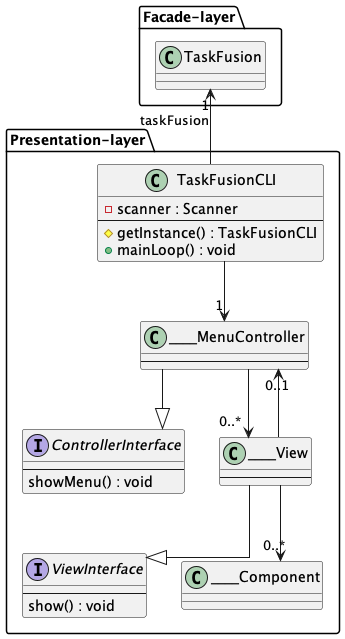
\includegraphics[width = 5cm, keepaspectratio]{TaskFusion/out/assets/diagrams/class_cli/TaskFusion-CLI.png}
    \label{fig:class_cli}
\end{figure}

\subsubsection{CLI brugergrænsefladen}
Da CLI grænsefladen til TaskFusion er opbygget af \textit{MenuController}'re og \textit{View}'s, ender vi da også med et netværk af mulige veje brugeren kan gå. For at få et overblik over TaskFusion, er herunder i \ref{fig:flow_cli} et \textit{flow}-diagram over menuer og sider i CLI grænsefladen. Diagrammet er ikke tiltænkt at være noteringsmæssig korrekt, men har fungeret effektivt som mockup i udviklgsfasen, og stadig til at skabe et overblik over programmet. En større version af figuren kan ses i appendix \ref{apdx:classDiagram_presentation}.
\begin{figure}[H]
    \centering
    \caption{Flowdiagram over CLI brugergrænsefladen}
    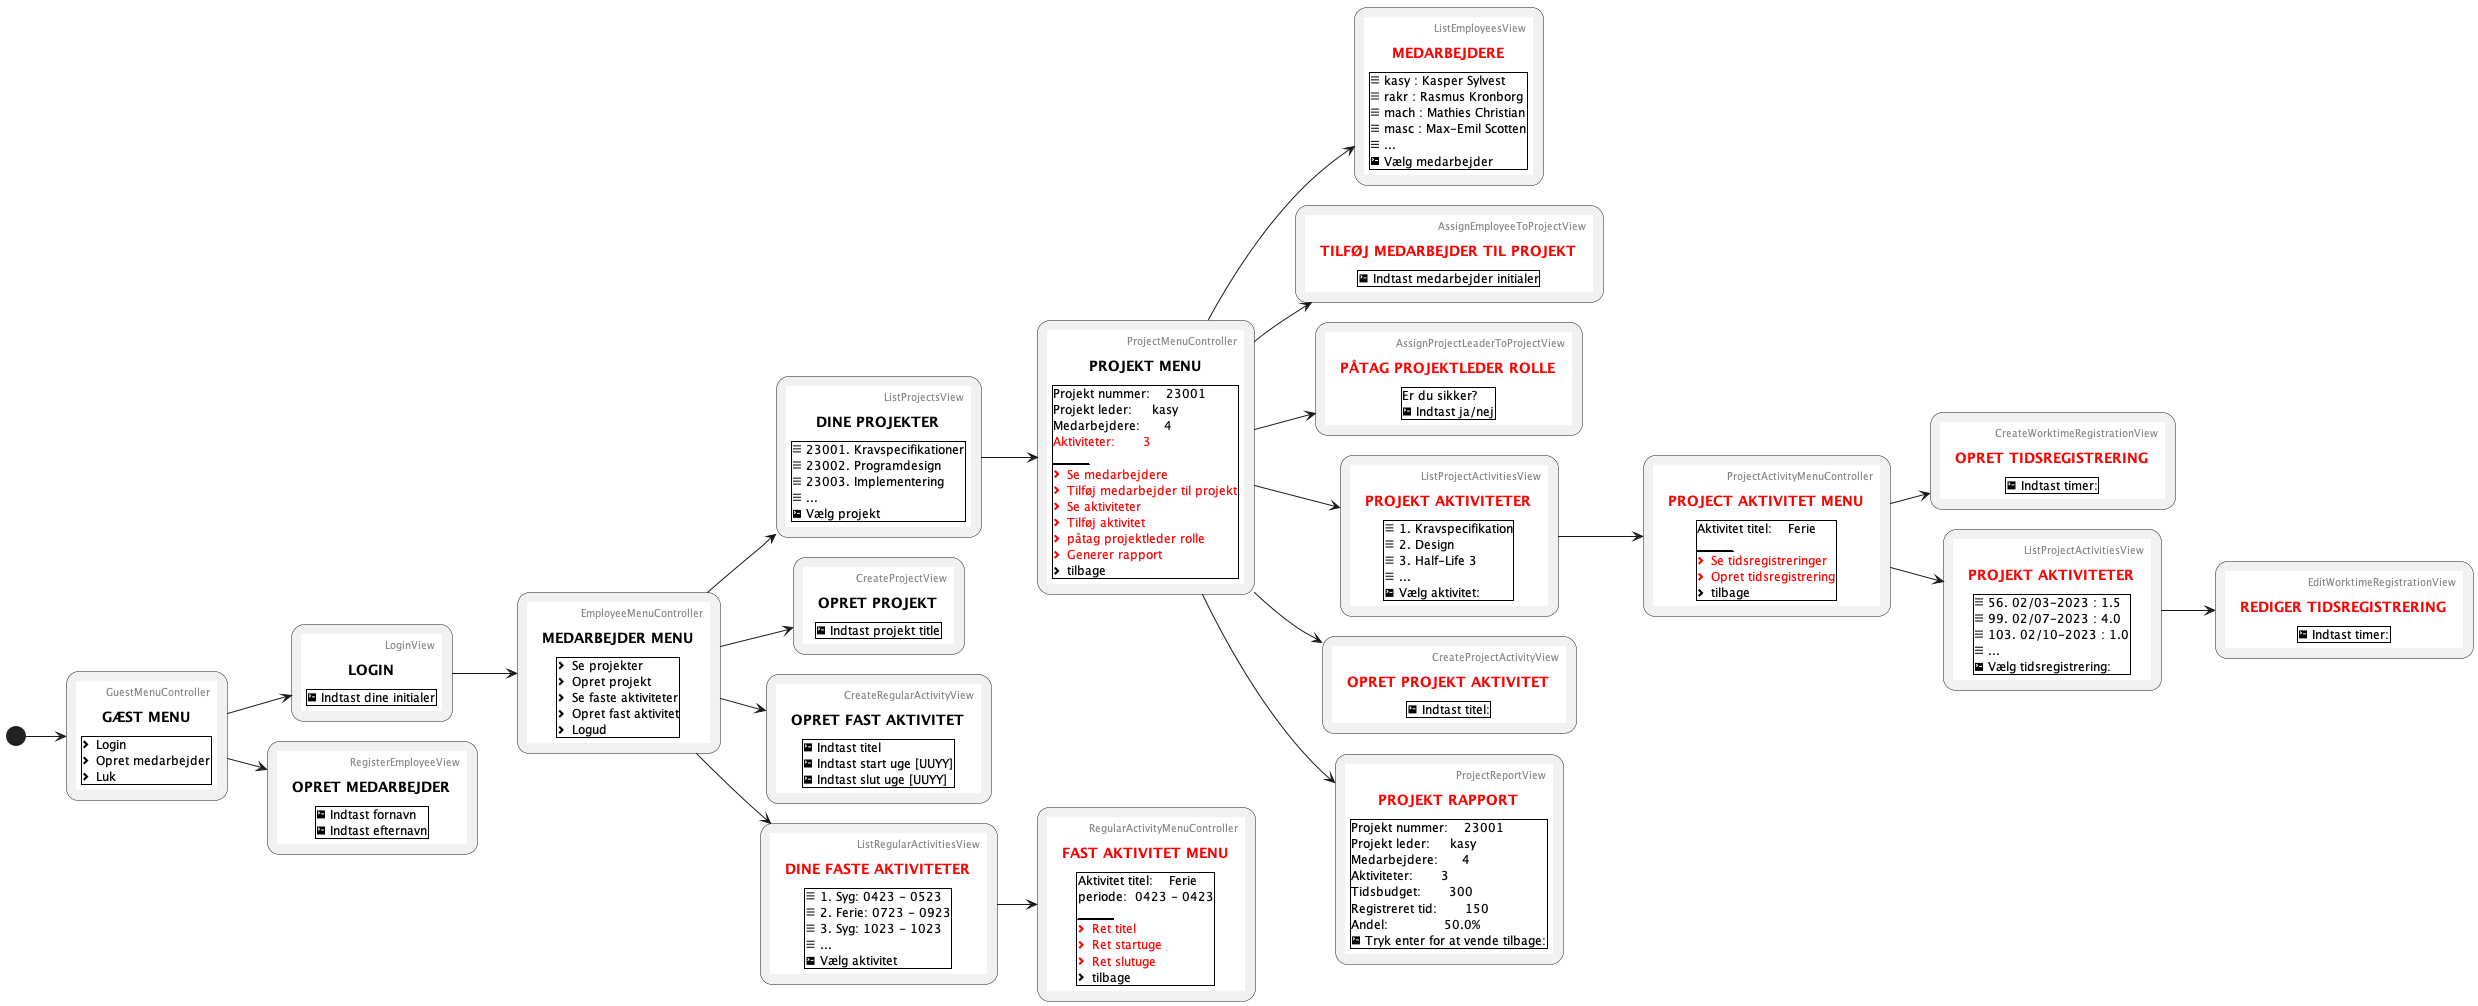
\includegraphics[width = \textwidth, keepaspectratio]{TaskFusion/out/assets/diagrams/flow_cli/flow_cli.png}
    \label{fig:flow_cli}
\end{figure}